%----------------------------------------------------------------------------------------
%	PACKAGES AND OTHER DOCUMENT CONFIGURATIONS
%----------------------------------------------------------------------------------------

%% maize2018 is A0
\documentclass[a0,30pt]{sciposter}
\usepackage[T1]{fontenc}
\usepackage[centertags]{amsmath}
\usepackage{amsfonts,multicol}
\usepackage{graphicx,colortbl}
\usepackage{hyperref}
\hypersetup{pdfpagelayout=SinglePage}
\pagestyle{plain}

%% sciposter handy command to set margins
\setmargins[30mm]

%% enable specifying colors by their 'svgnames', for a full list of all colors available see here: http://www.latextemplates.com/svgnames-colors
\usepackage{fontspec}
\usepackage[svgnames]{xcolor}

%% Carnegie uses Roboto Slab (serif) and Lato (sans serif)
\setmainfont[Ligatures=TeX]{Lato}

%% Carnegie colors
\definecolor{CarnegiePriBlue}{cmyk}{1.00,0.85,0.15,0.25}  % main primary blue
\definecolor{CarnegieSecBlue1}{cmyk}{0.68,0.48,0.00,0.00} % first secondary blue
\definecolor{CarnegieSecBlue2}{cmyk}{0.85,0.69,0.04,0.00} % second secondary blue
\definecolor{CarnegiePriTurq}{cmyk}{0.60,0.10,0.15,0.00}  % main primary turquoise
\definecolor{CarnegiePriGreen}{cmyk}{0.46,0.00,0.90,0.00} % main primary green
\definecolor{CarnegiePriBrown}{cmyk}{0.25,0.40,0.65,0.00} % main primary brown

%% multiple columns
\usepackage{multicol} % This is so we can have multiple columns of text side-by-side
\columnsep=100pt      % This is the amount of white space between the columns in the poster
\columnseprule=3pt    % This is the thickness of the black line between the columns in the poster
\def\columnseprulecolor{\color{lightgray}}

%% other needed packages
\usepackage{amsfonts, amsmath, amsthm, amssymb} % For math fonts, symbols and environments
\usepackage{wrapfig}  % Allows wrapping text around tables and figures
\usepackage{graphicx} % Required for including images
\usepackage{booktabs} % Top and bottom rules for table

%% tweak figure and table captions
\usepackage[font=small,labelfont={bf,color=CarnegiePriBlue},textfont={color=CarnegiePriBlue},margin=0pt,skip=18pt]{caption}

%% natbib drops numbers and we'll shrink text size; drop labels
\usepackage{natbib}
\def\bibfont{\footnotesize}
\makeatletter
\renewcommand\@biblabel[1]{}
\makeatother

%% tweak list spacing
\usepackage{enumitem}
\setlist[itemize]{topsep=10pt,itemsep=8pt,itemindent=48pt}
\setlist[enumerate]{topsep=10pt,itemsep=8pt,itemindent=0pt}

%% tweak paragraphs
\setlength{\parindent}{0pt}
\setlength{\parskip}{12pt}

%% tweak title spacing and colors
\usepackage{titlesec}
%% \titlespacing{command}{left spacing}{before spacing}{after spacing}[right]
%% spacing: how to read {12pt plus 4pt minus 2pt}
%%          12pt is what we would like the spacing to be
%%          plus 4pt means that TeX can stretch it by at most 4pt
%%          minus 2pt means that TeX can shrink it by at most 2pt
%% {left}{before}{after}
\titlespacing{\section}{0pt}{36pt}{12pt}
\titlespacing{\subsection}{0pt}{12pt}{12pt}
\titlespacing{\subsubsection}{0pt}{12pt}{12pt}
\titleformat{\section}{\color{CarnegiePriBlue}\Large\bfseries}{\color{CarnegiePriBlue}\thesection}{1em}{}
\titleformat{\subsection}{\color{CarnegiePriBrown}\large\bfseries}{\color{CarnegiePriBrown}\thesubsection}{1em}{}

%% tweak equation whitespace
% \abovedisplayskip=12pt plus 3pt minus 9pt
% \abovedisplayshortskip=0pt plus 3pt
% \belowdisplayskip=12pt plus 3pt minus 9pt
% \belowdisplayshortskip=7pt plus 3pt minus 4pt

%% width of figures for consistency
\newlength{\figwidth}
\setlength{\figwidth}{1.90\linewidth}

%% space above figures
\newlength{\figtopspace}
\setlength{\figtopspace}{10pt}

%% location of the graphics files
\graphicspath{{figures/}}

%% DEBUG: overlay a grid to view spacing
%\usepackage[grid,gridcolor=red!20,subgridcolor=green!20,gridunit=in]{eso-pic}

\begin{document}

%%----------------------------------------------------------------------------------------
%%	POSTER HEADER 
%%----------------------------------------------------------------------------------------

%% The header is divided into three boxes:
%% Note: no line breaks between minipage environments!

%% Title
%% Use an explicit font size to get the title to stretch nicely across the full width
\textbf{\color{CarnegiePriBlue} \fontsize{72}{12}\selectfont Transcriptomic characterization of male sexual reproduction in maize}

\begin{minipage}[m]{0.12\linewidth}
  
\includegraphics[height=75mm]{oregon-state-vert.png}
\end{minipage}
\begin{minipage}[m]{0.25\linewidth}
  \color{Black}
  \Large
  \textbf{Zuzana Vejlupkova \\ Rex A Cole \\ John E Fowler \\ \underline{Matthew Warman}}
  \hfill
\end{minipage}
\begin{minipage}[m]{0.12\linewidth}
  
\includegraphics[height=75mm]{CS_plantbio_logo_vert.eps}
\end{minipage}
\begin{minipage}[m]{0.19\linewidth}
  \color{Black}
  \Large
  \textbf{\underline{Sam Hokin} \\ Matt Evans}
  \hfill
\end{minipage}
\begin{minipage}[m]{0.15\linewidth}
  
\includegraphics[height=75mm]{ohio-state-vert.png}
\end{minipage}
\begin{minipage}[m]{0.15\linewidth}
  \color{Black}
  \Large
  \textbf{Kaushik Panda \\ R. Keith Slotkin}
  \hfill
\end{minipage}

\vspace{5mm} % A bit of extra whitespace between the header and poster content

%% horizontal line
\color{CarnegiePriBlue}
\hrulefill

%% default text color
\color{Black}

%% This is how many columns your poster will be broken into, a poster with many figures may benefit from less columns whereas a text-heavy poster benefits from more
\begin{multicols}{3}
  
  %----------------------------------------------------------------------------------------
  %	INTRODUCTION
  %----------------------------------------------------------------------------------------

  \section*{INTRODUCTION}

  Sexual reproduction in plants involves developmental regulation of key cellular processes (e.g., pollen tube growth, cell-cell signaling, fertilization). Recent results demonstrate 
  that plant genomes undergo large scale alteration of gene expression and epigenetic modifications as plants undergo meiosis to produce haploid gametophytes for the next generation.
  \textbf{We have undertaken a transcriptomic study of male sexual development in maize to investigate these regulatory events.}
  
  \section*{REPRODUCTIVE TISSUES}
  
  \begin{center}
    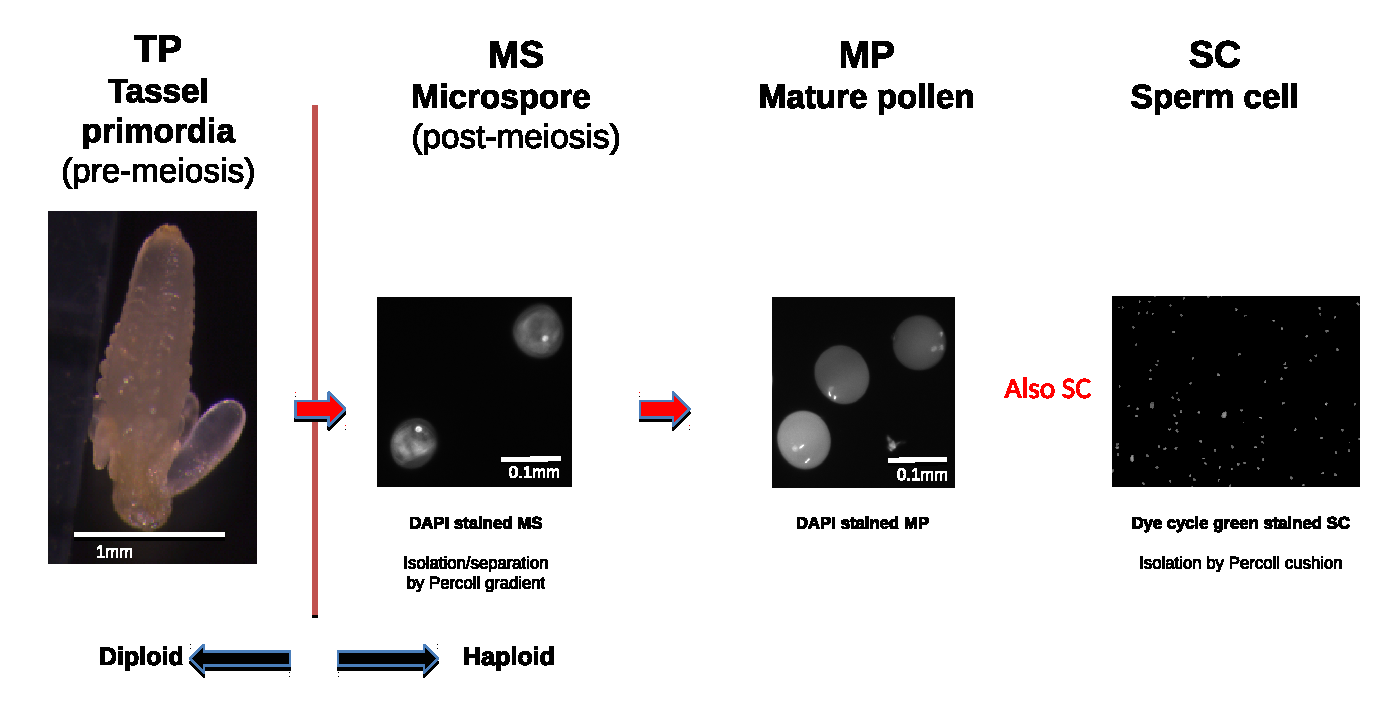
\includegraphics[width=\figwidth]{Samples-Libraries.eps}
    \captionof*{figure}{
      We developed methods to isolate and sequence paired samples of mRNA and small RNA from each of four biological replicates at four developmental stages.
    }
  \end{center}

  \section*{RNA SEQUENCING}

  \begin{center}
    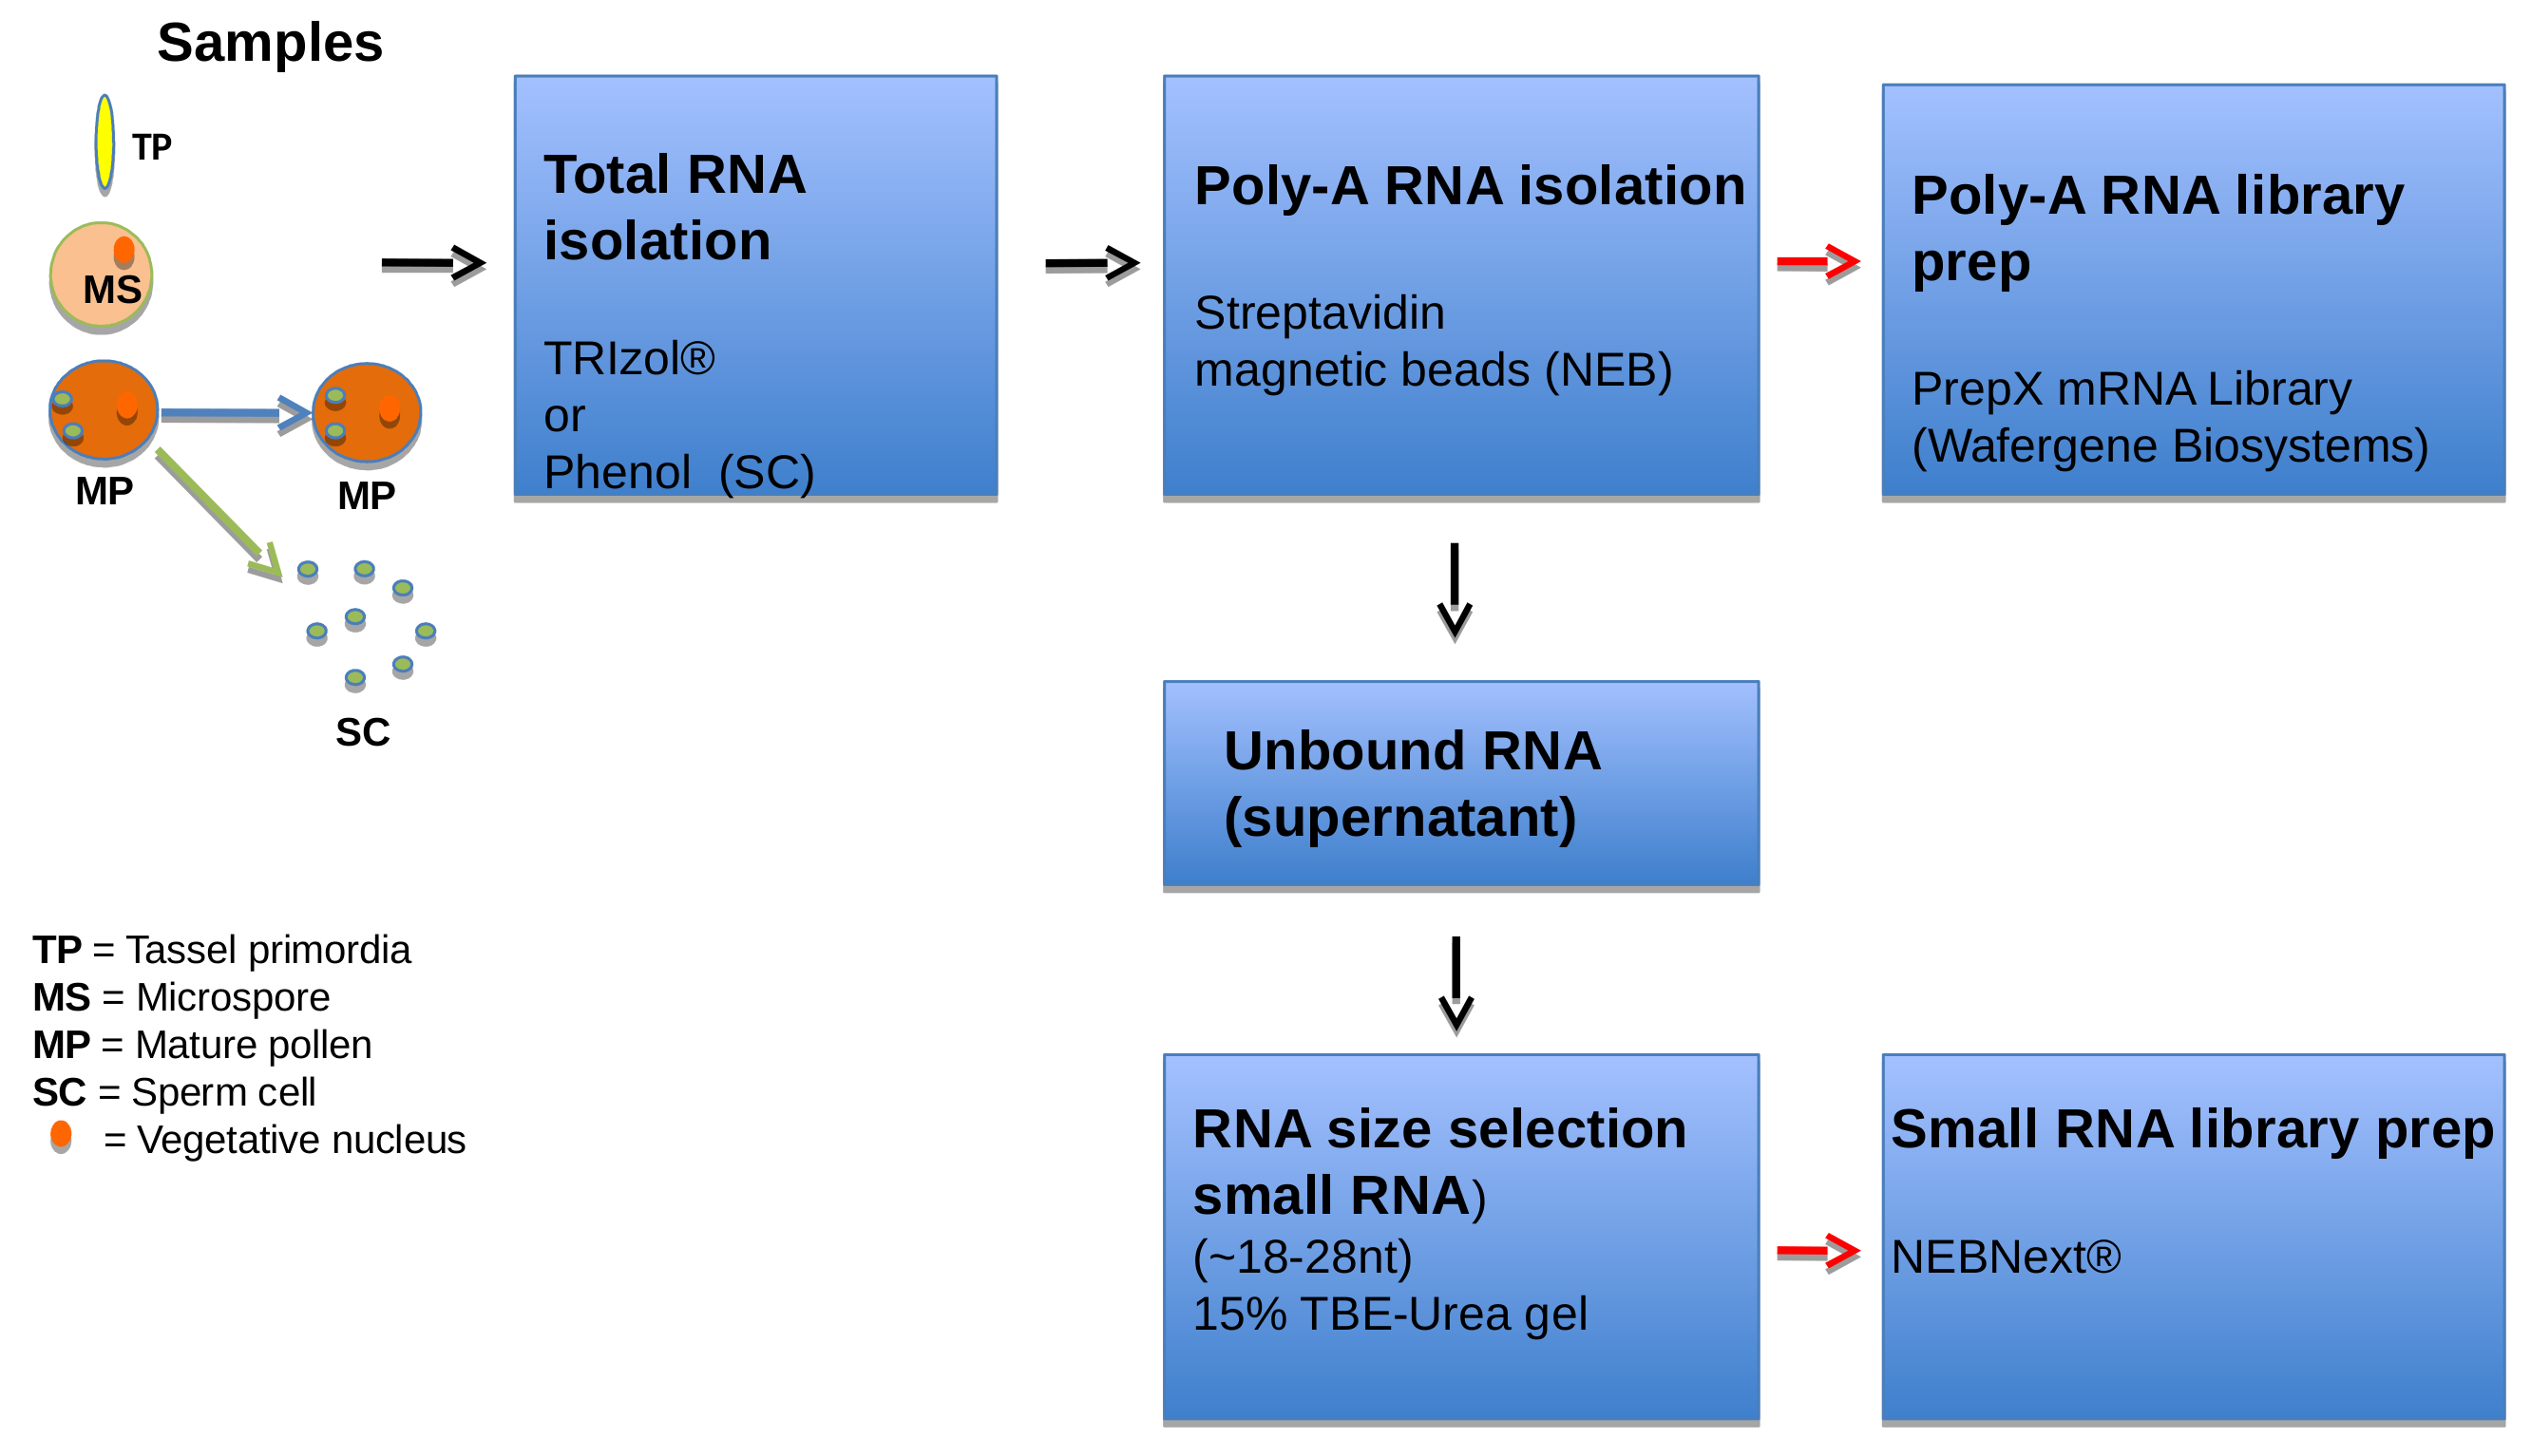
\includegraphics[width=\figwidth]{sequencing-prep.png}
    \captionof*{figure}{
      Mature pollen (MP) and sperm cell (SC) samples were isolated from the same pollen sample that was a pool of pollen from 3 plants.
      Part of each pool was used for MP RNA isolation and part was used for SC RNA isolation.
      All of the samples were used for both poly-A RNA and small RNA sequencing.
    }
  \end{center}

  \subsection*{PCA analysis}

  PCA analysis of the datasets indicate that replicates from each tissue have low variance, enabling statistical confirmation of
  differential expression of genes or transposable elements observed between tissues.

  Our mature pollen (MP) sequencing datasets resemble previously sequenced high-quality datasets.

  \begin{center}
    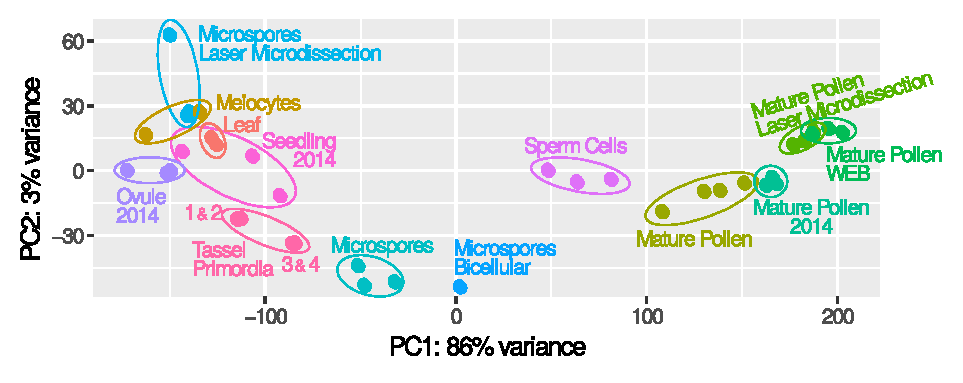
\includegraphics[width=\figwidth]{PCA.eps}
    \captionof*{figure}{
      PCA plots show the quality of our reproducible RNA-seq datasets when assaying non-TE gene expression.
      Note that the vast majority of variance is on the X-axis. Also note the clustering of our Mature Pollen samples with those already published in the field:
      `* 2014' = Chettoor, et al. (2014); `WEB' = Walley, et al. (2016); `Laser Microdissection' = NCBI BioProject 306885 (2015).
    }
  \end{center}

  \subsection*{Highly-expressed genes}
  
  \begin{center}
    \begin{minipage}[t]{0.5\figwidth}
      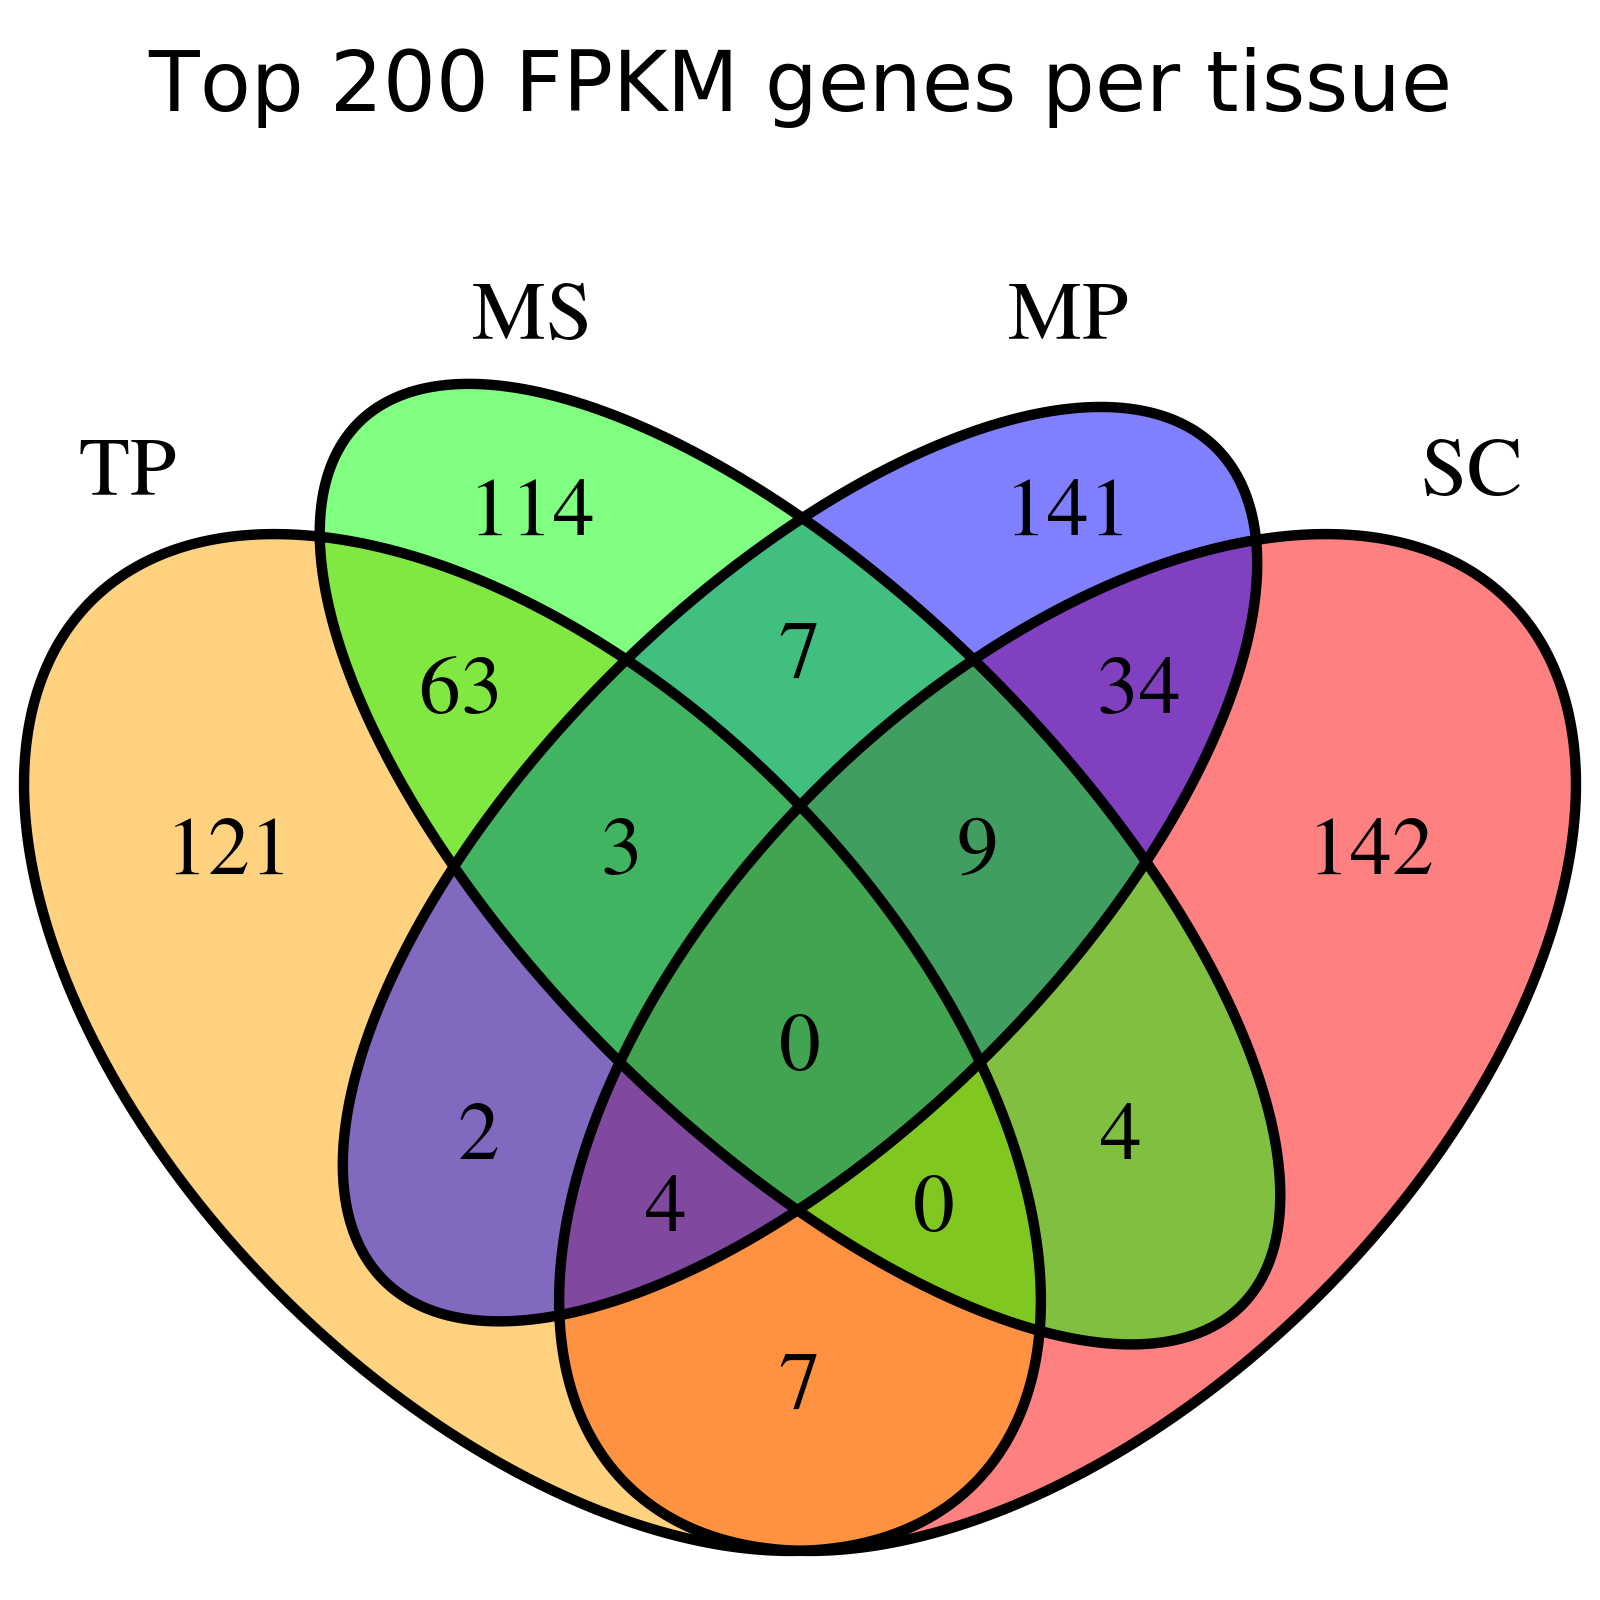
\includegraphics[width=0.47\figwidth]{Fowler-top200-Venn.png}
    \end{minipage}
    \begin{minipage}[b]{0.5\figwidth}
      \captionof*{figure}{
        High expression levels are associated with developmental specificity: approximately 2/3 of the genes associated with the highest FPKM values in each of the four sample types are
        highly expressed in only that sample type.
      }
    \end{minipage}
  \end{center}
  
  Consistent with the PCA analysis, overlaps in highly-expressed genes suggests that mature pollen (MP) and sperm cells (SC) are more similar,
  and distinct from the tassel primordia (TP) and microspore (MS) pairing.

  \subsection*{GO enrichment}
  
  Gene ontology (GO) analysis of mRNA transcripts highlights contrasting cellular processes in mature pollen (containing sperm cells as well as the vegetative cell) and sperm cells alone,
  consistent with the distinct roles of the sperm cells and the vegetative cell in reproduction.

  \begin{center}
    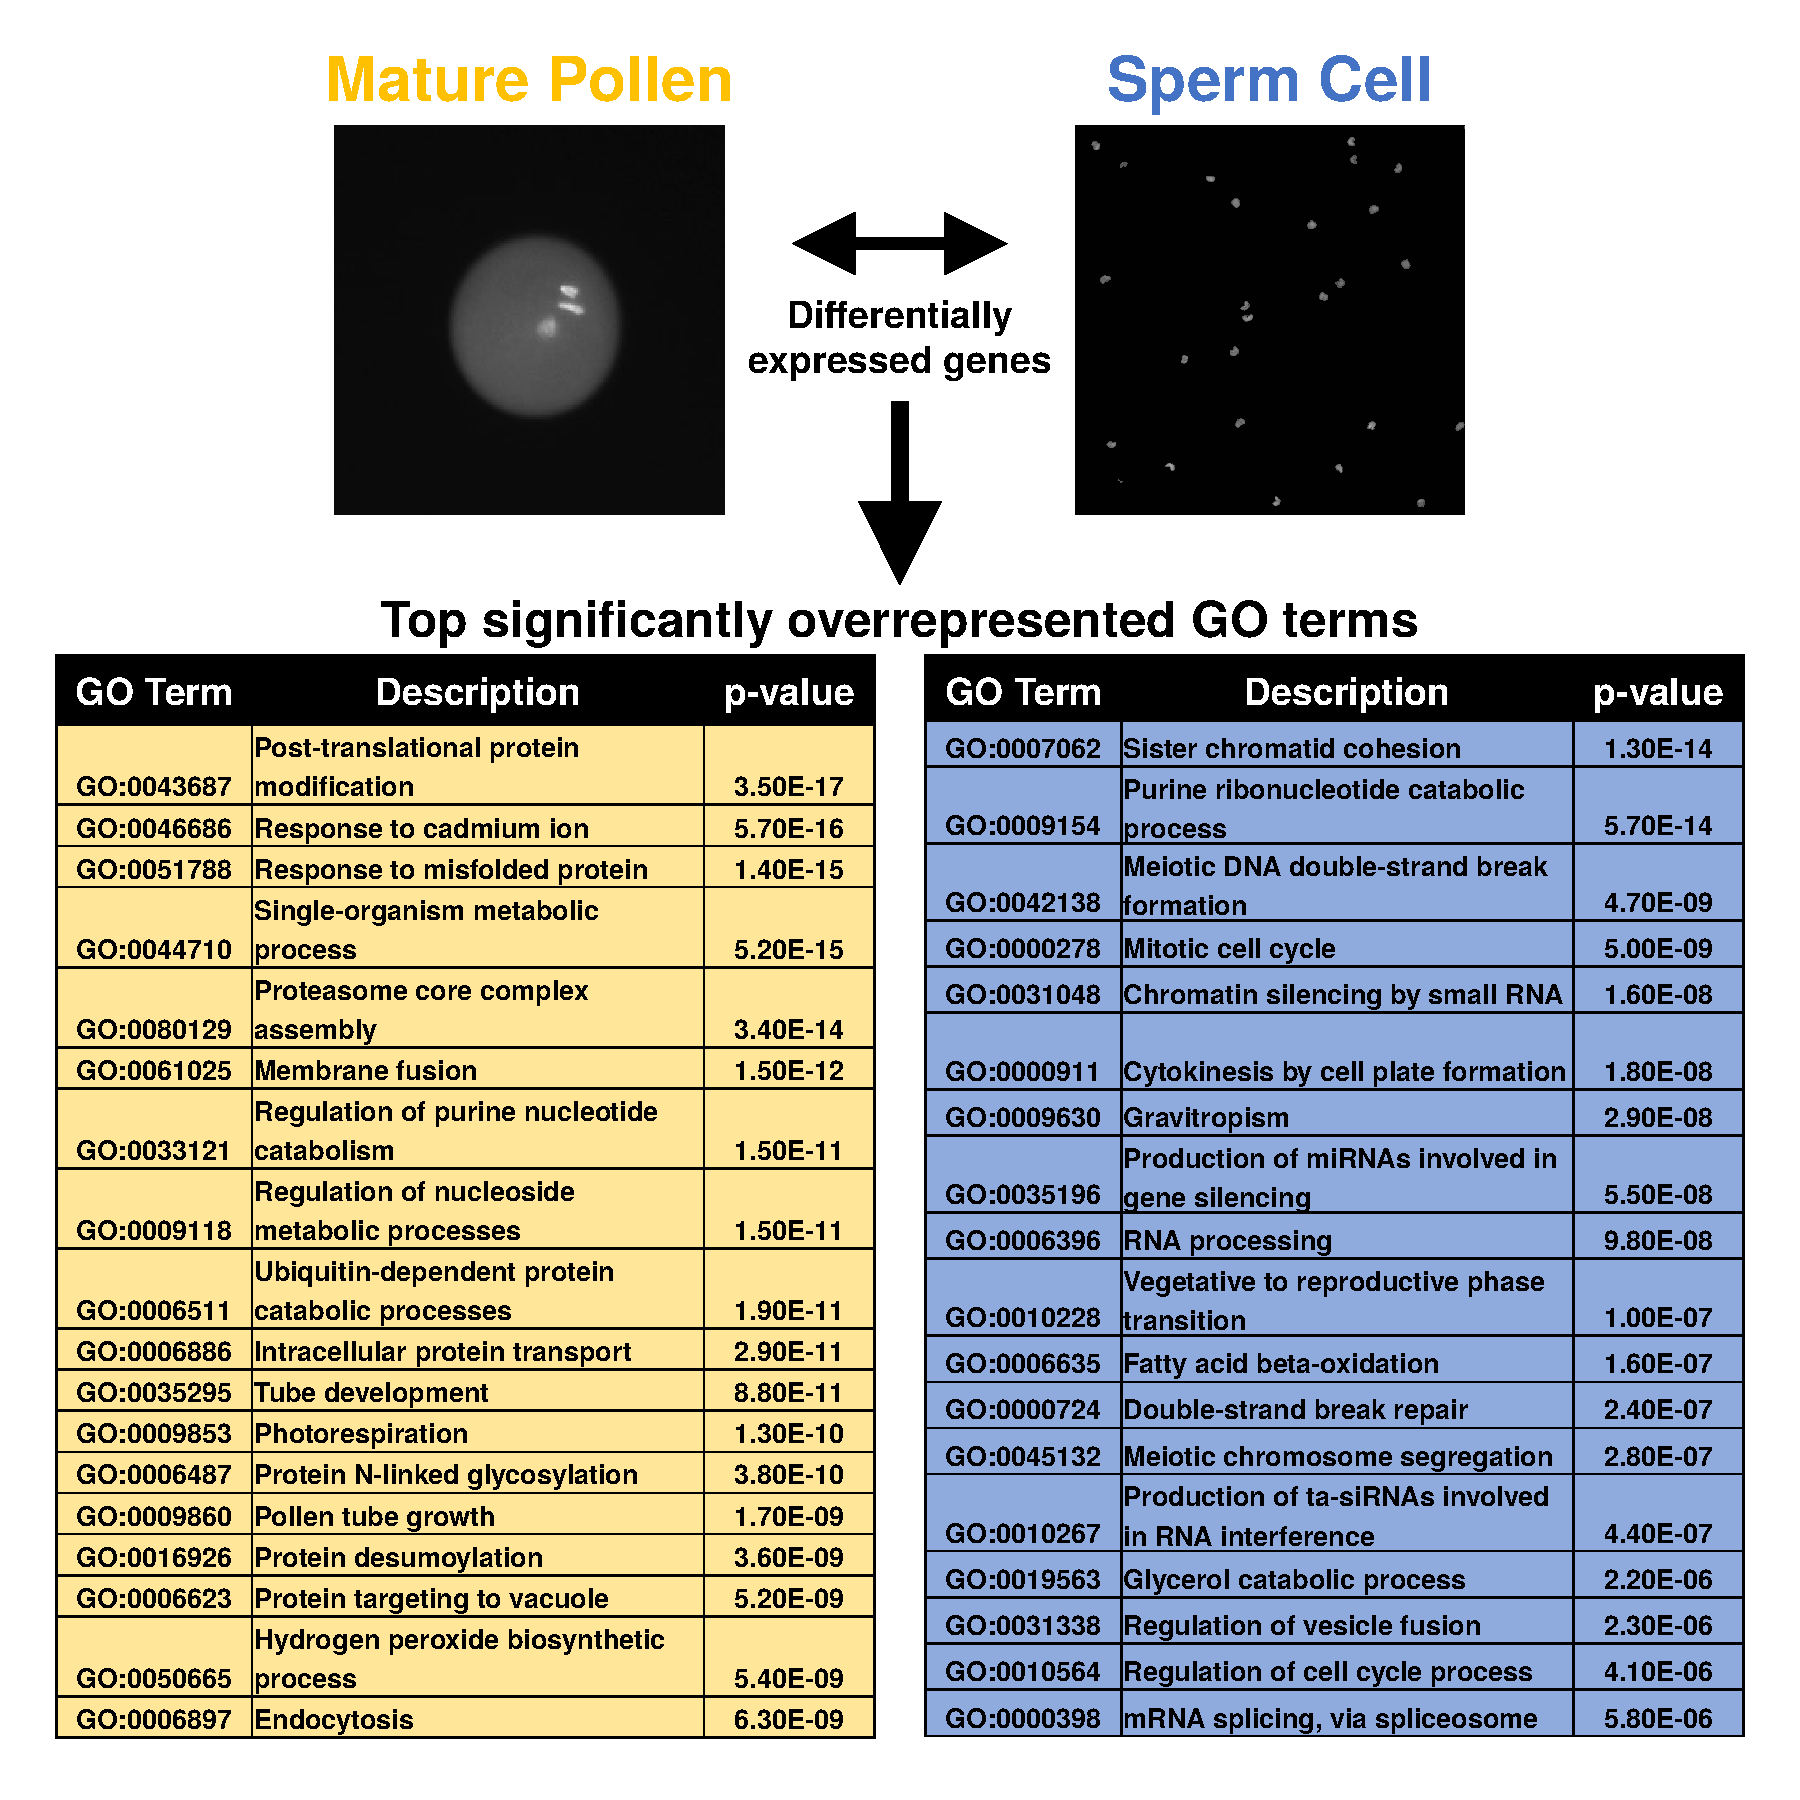
\includegraphics[width=\figwidth]{MP-SC-GO-enrichment.pdf}
    \captionof*{figure}{
      GO annotations were assigned to highly differentially expressed genes ($q<0.01$) using the R package \texttt{topGO} (Alexa, 2016) in combination with maize-GAMER,
      a recent maize gene functional annotation (Wimalanathan, 2017).
      GO annotations associated with genes highly-expressed in mature pollen are shown in yellow, while those associated with genes highly-expressed in sperm cells are shown in blue.
    }
  \end{center}
  

  \subsection*{Dynamic TE regulation}

  \begin{center}
    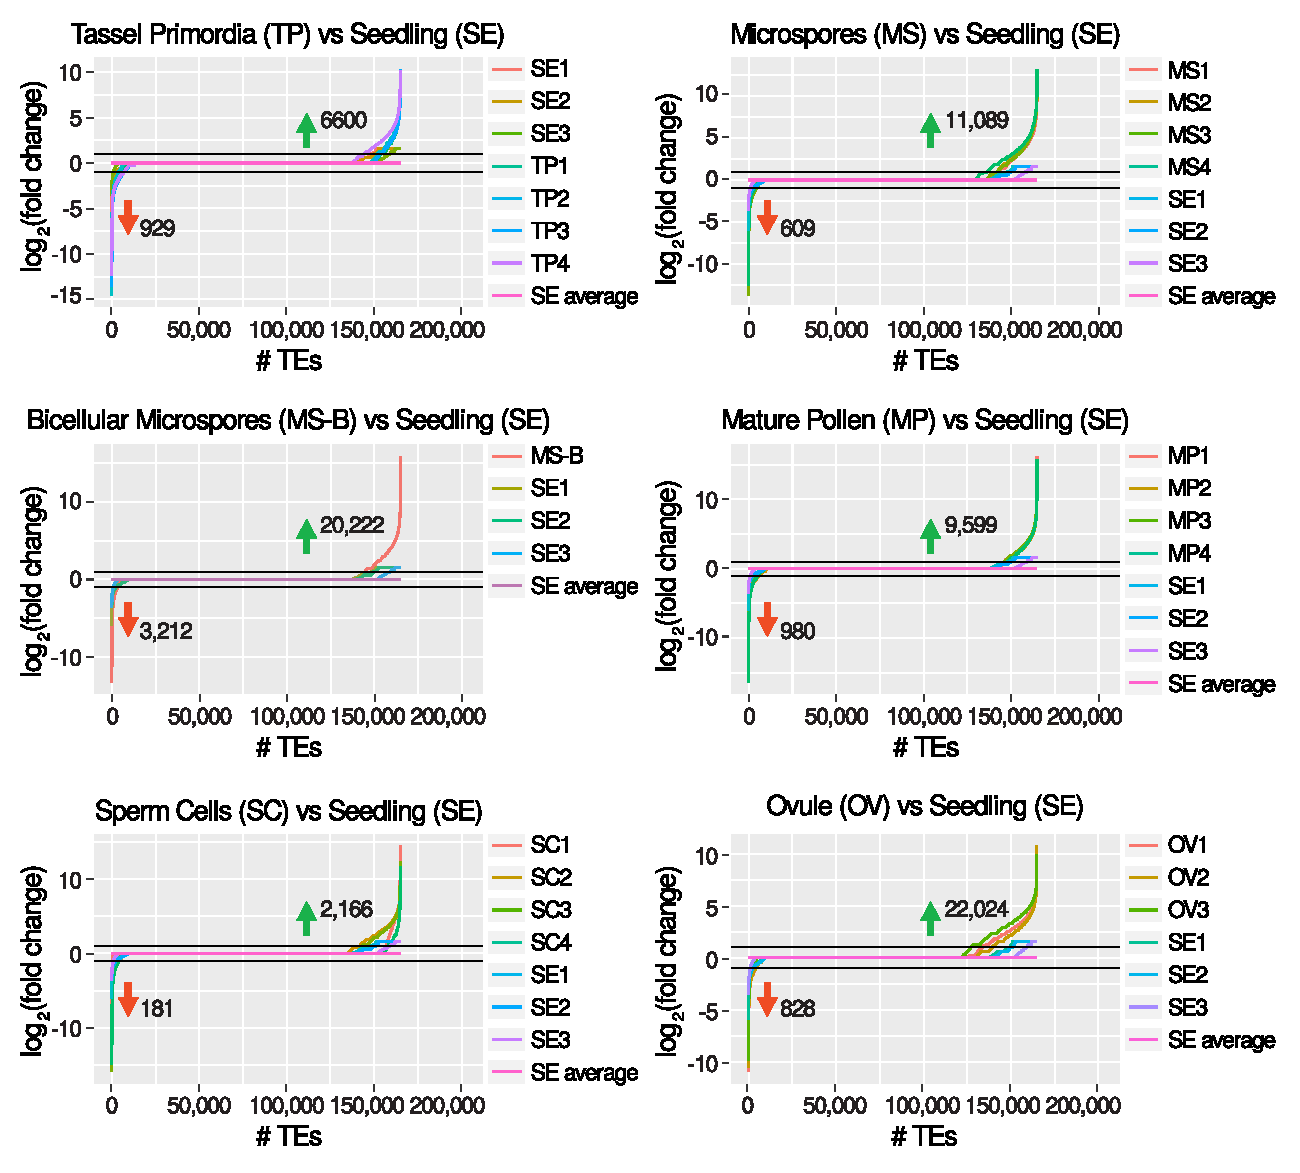
\includegraphics[width=\figwidth]{TE-up-regulation.eps}
    \captionof*{figure}{
      Compared to the baseline TE expression in seedlings, TEs are up-regulated in Tassel Primordia through Mature Pollen development.
      Most of these are not expressed in Sperm Cells. On the female side, we see many TEs up-regulated in ovules as well.
      We are only considering TEs farther than 2kb from genes and hence, read-through transcription from developmental changes in gene expression
      should not be an underlying cause for the observed dynamic behavior of TEs.
    }
  \end{center}
  
  \begin{center}
    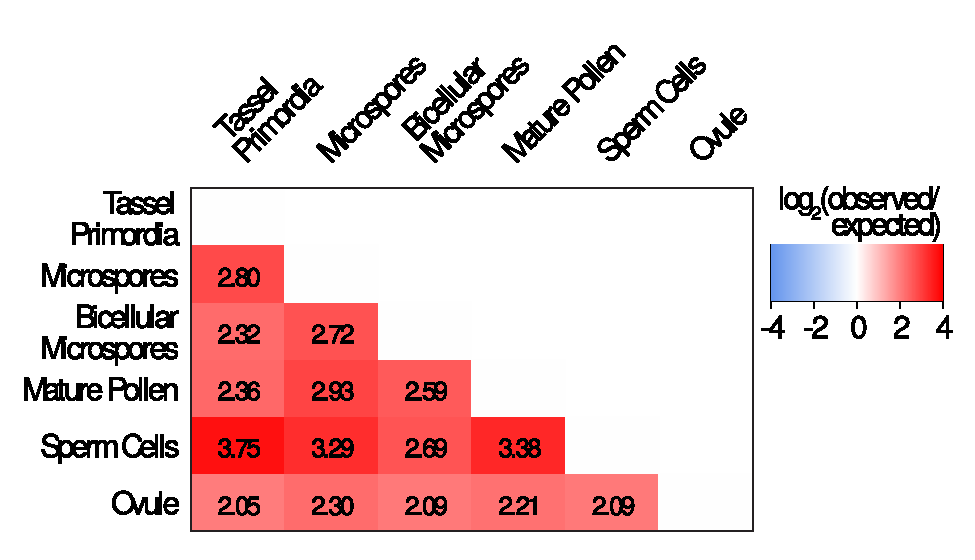
\includegraphics[width=\figwidth]{TE-overlap.eps}
    \captionof*{figure}{
      There is significant overlap between the sets of TEs that are up-regulated at specific stages of maize reproductive development.
      This demonstrates that there are a class of TEs that are dynamically and specifically up-regulated on both the male and female side during maize reproduction.
    }
  \end{center}
  
  To better assess dynamic transposable element regulation in maize male reproductive tissues, we developed a bioinformatic tool to easily visualize and identify differentially-expressed
  transposable elements in these samples. Intriguingly, genes that are highly-expressed in either mature pollen or sperm cells are associated with fewer transposable element insertions in
  exons in sequenced populations (UniformMu, Photosynthetic Mutant Library), relative to highly-expressed seedling genes.
  This is consistent with the idea that deleterious mutations in genes important for either pollen or sperm cell function are subject to relatively higher purifying selection, likely due to the haploid 
  nature of these stages.

  \subsection*{Mu insertions}

  \begin{center}
    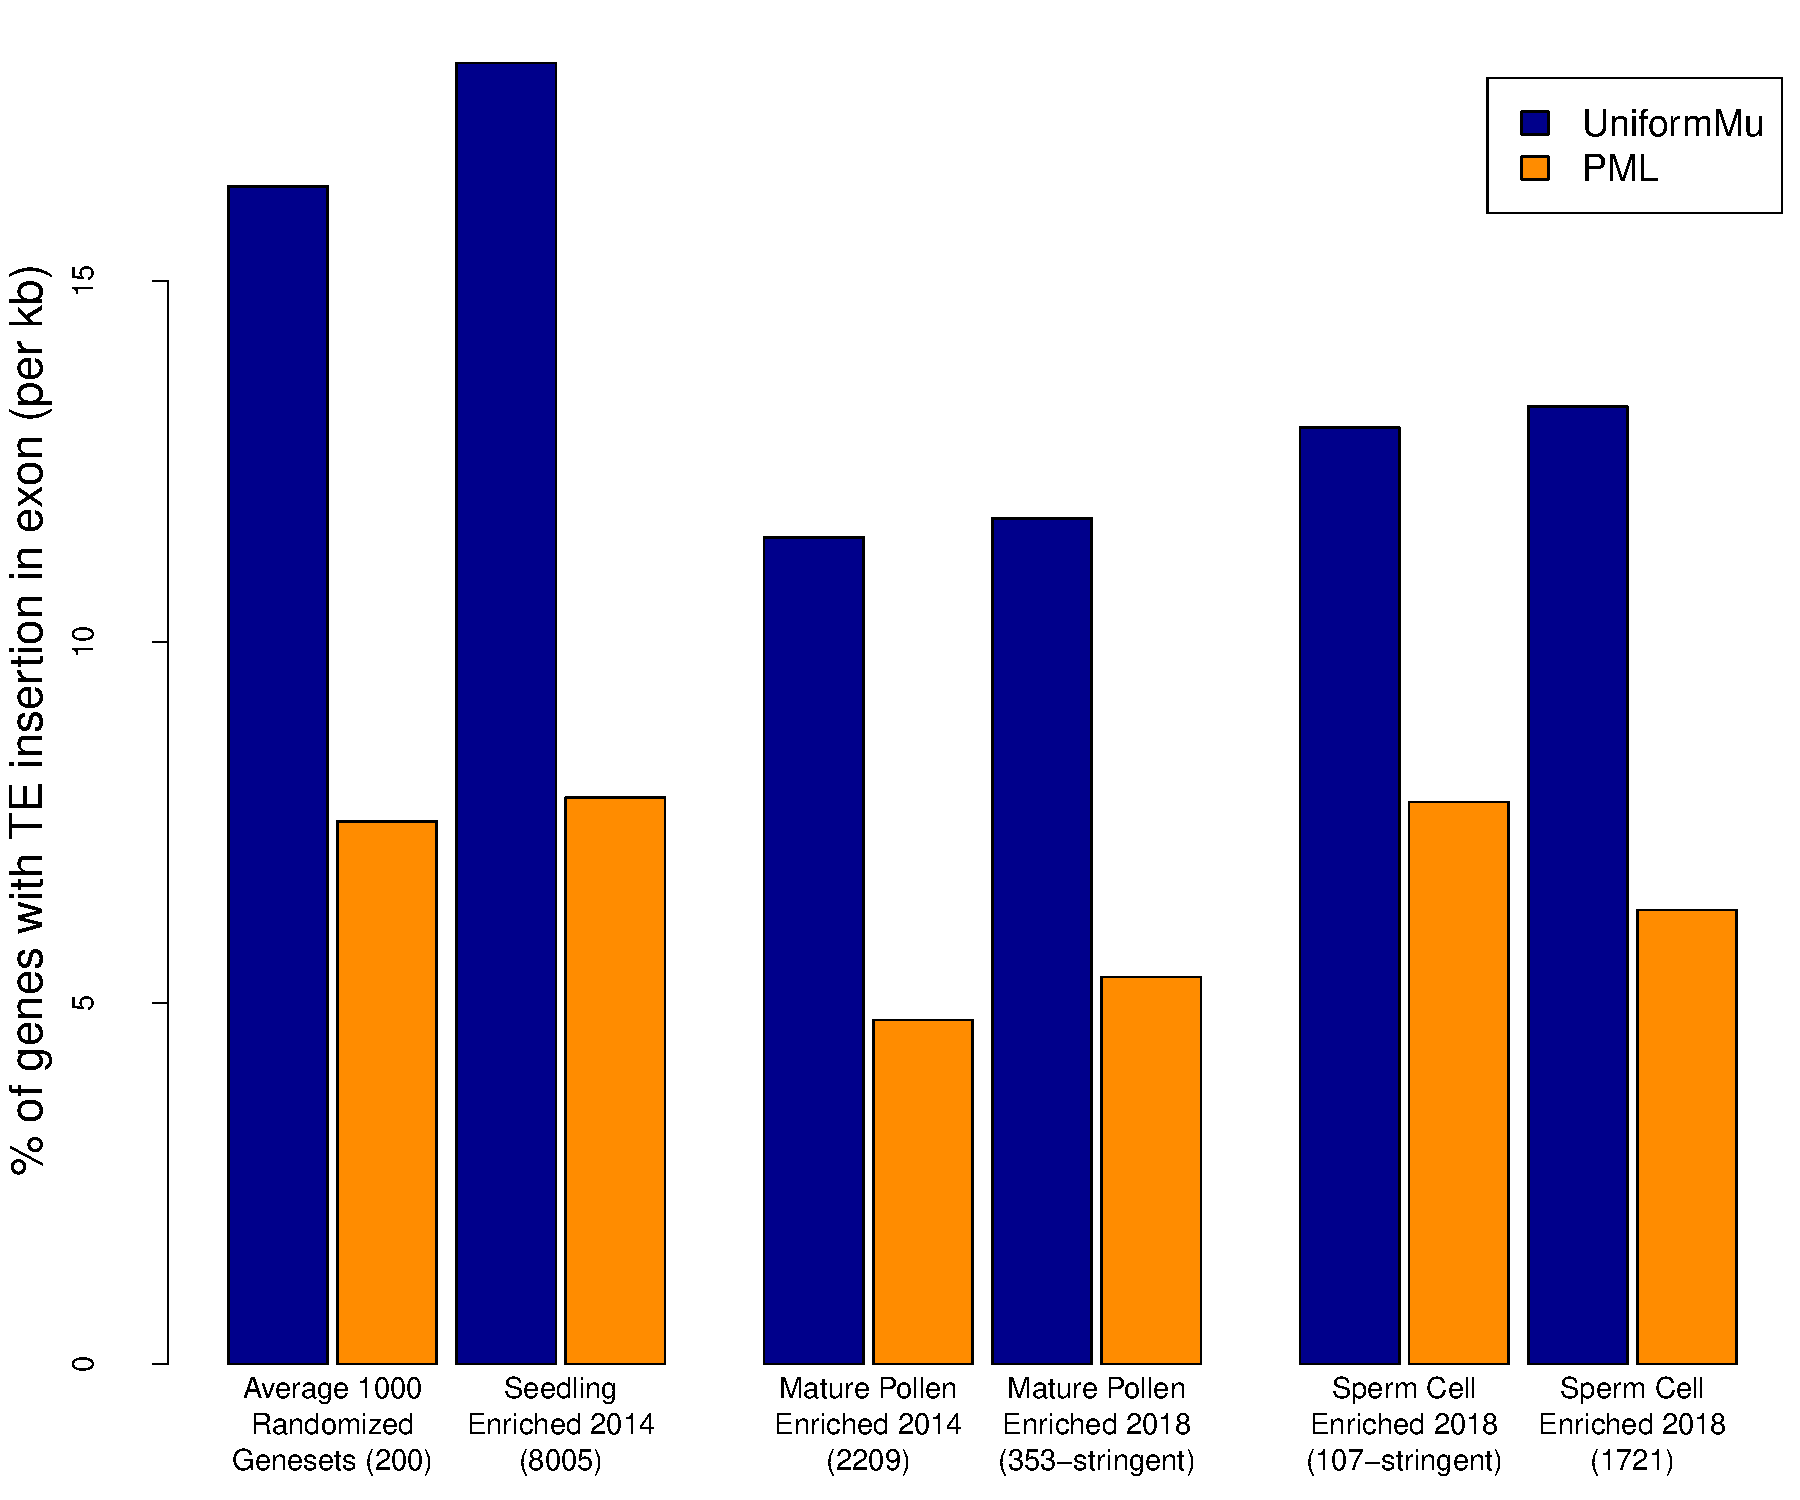
\includegraphics[width=\figwidth]{rrm-barplot.pdf}
    \captionof*{figure}{
      In two large populations (UniformMu and Photosynthetic Mutant Library), gene sets based on transcript enrichment in mature pollen and sperm cells are associated with
      reduced likelihood of Mu insertion sites in exons, relative to comparators.
      This is consistent with the hypothesis that these genesets are enriched for genes important during the haploid phase, as selection would reduce recovery of deleterious gametophyte mutations.
      Gene sets are based on data from Chettoor, et al. (2014) and this study (marked 2018); number in parenthesis is the number of genes in each set.
      Comparators are either seedling-enriched genes, or an average of percentages from 1000 randomized 200-member genesets.
    }
  \end{center}

  
  \section*{CONCLUSIONS}

  Maize provides a useful model for the regulation of transposon expression in a model system in which many transposon classes are still active.
  Analysis of a time course of male reproductive developmental using paired RNA-seq and sRNA-seq reveals changes in the regulation of transposon expression during the transition from the
  sporophytic phase to the gametophytic phase to the germ cells.  This analysis also provides a list of genes and pathways that are important to the whole male
  gametophyte and the sperm cells specifically.

  Further analysis of how regulation of expression of the transposon landscape is coordinated with expression of the
  functional genes during gametophyte development is an important area for future research.
  
  %----------------------------------------------------------------------------------------
  %	REFERENCES
  %----------------------------------------------------------------------------------------

  \nocite{*} % Print all references regardless of whether they were cited in the poster or not
  \bibliographystyle{plain} % Plain referencing style
  \bibliography{mgp-maize2018} % Use mgp-maize2018.bbl - regenerate with bibtex

  %----------------------------------------------------------------------------------------
  %	ACKNOWLEDGEMENTS
  %----------------------------------------------------------------------------------------

  {\small\color{CarnegiePriBrown} This research was funded by NSF award \#0701731.}

\end{multicols}
\end{document}
